
\documentclass[conference]{IEEEtran}

\usepackage{graphicx}
\usepackage{hyperref}
%\usepackage{caption}
%\usepackage{subcaption}

%\usepackage[turnoff]{notes}
\usepackage[turnon]{notes}

\begin{document}

\title{Virtual Reality in Software Engineering: Affordances, Applications, and Challenges}

\author{\IEEEauthorblockN{Anthony Elliott}
\IEEEauthorblockA{Department of Computer Science\\
North Carolina State University\\
Raleigh, North Carolina, USA\\
anthony\_elliott@ncsu.edu}
\and
\IEEEauthorblockN{Brian Peiris}
\IEEEauthorblockA{Toronto, Ontario, Canada\\
brian@peiris.io}
\and
\IEEEauthorblockN{Chris Parnin}
\IEEEauthorblockA{Department of Computer Science\\
North Carolina State University\\
Raleigh, North Carolina, USA\\
chris.parnin@ncsu.edu}}

\maketitle
\begin{abstract}
Software engineers primarily interact with software using a keyboard and mouse and typically view software on three or fewer monitors.
This interaction paradigm does not take advantage of many affordances of natural human movement and perception.
Virtual reality (VR) environments designed for software engineering could greatly increase productivity by taking advantage of innate affordances.
This paper describes several prototype applications for software engineering tools in VR, including a live coding environment and code review system, and discusses possible benefits, open research questions, challenges, and future research directions.
\end{abstract}

\section{Introduction}

Programming environments have not significantly changed in decades, 
despite advances in psychology, neuroscience, and social aspects of software development.
As a result, problems still persist.  Developers still experience disorientation when navigating code~\cite{Henley:2014}.
Developers still experience problems comprehending code~\cite{Maalej:TOSEM:2014}.  These basic issues also impede other important software engineering activities. For example,
when performing a code review, developers mostly report issues, such as code convention violations, instead of discussing design flaws or defects
due to insufficient ability to navigate and understand the code under review~\cite{bacchelli:ModernCodeReviewChallenges}.  
%Other challenges, such as remote pairing, still persist.

%The primary reason for modern code reviews not resulting in more defects found is a lack of understanding of the code being modified~\cite{bacchelli:ModernCodeReviewChallenges}. 
Researchers have explored the underlying cognitive issues to several problems developers experience~\cite{Parnin:2012}.
For example, \emph{spatial memory}, a memory system in the parahippocampus that supports ability to retain memory of locations, is supported by place cells that fire as a person navigates through a physical space and other contextual cues in the environment.  Even after a single exposure, these memories can persist as long as a year.  The disorientation developers experience often result from failures to engage a human's innate processing of spatial memory. Ko et al.~\cite{Ko:2006} observed that developers lost track of relevant code because they had to temporarily navigate to another location and forgot how to find the original location. This loss was because the cues they relied on, such as position of scroll bars and document tabs, were unstable or disrupted as a result of their navigation.  Kuhn~\cite{Kuhn:2010} describes how developers maintain an internal spatial representation of code, and refer to code as being ``above or below'' another.

\begin{figure}[ht]
\centering
%\begin{subfigure}{.5\columnwidth}
%	\centering
\begin{tabular}{cc}
	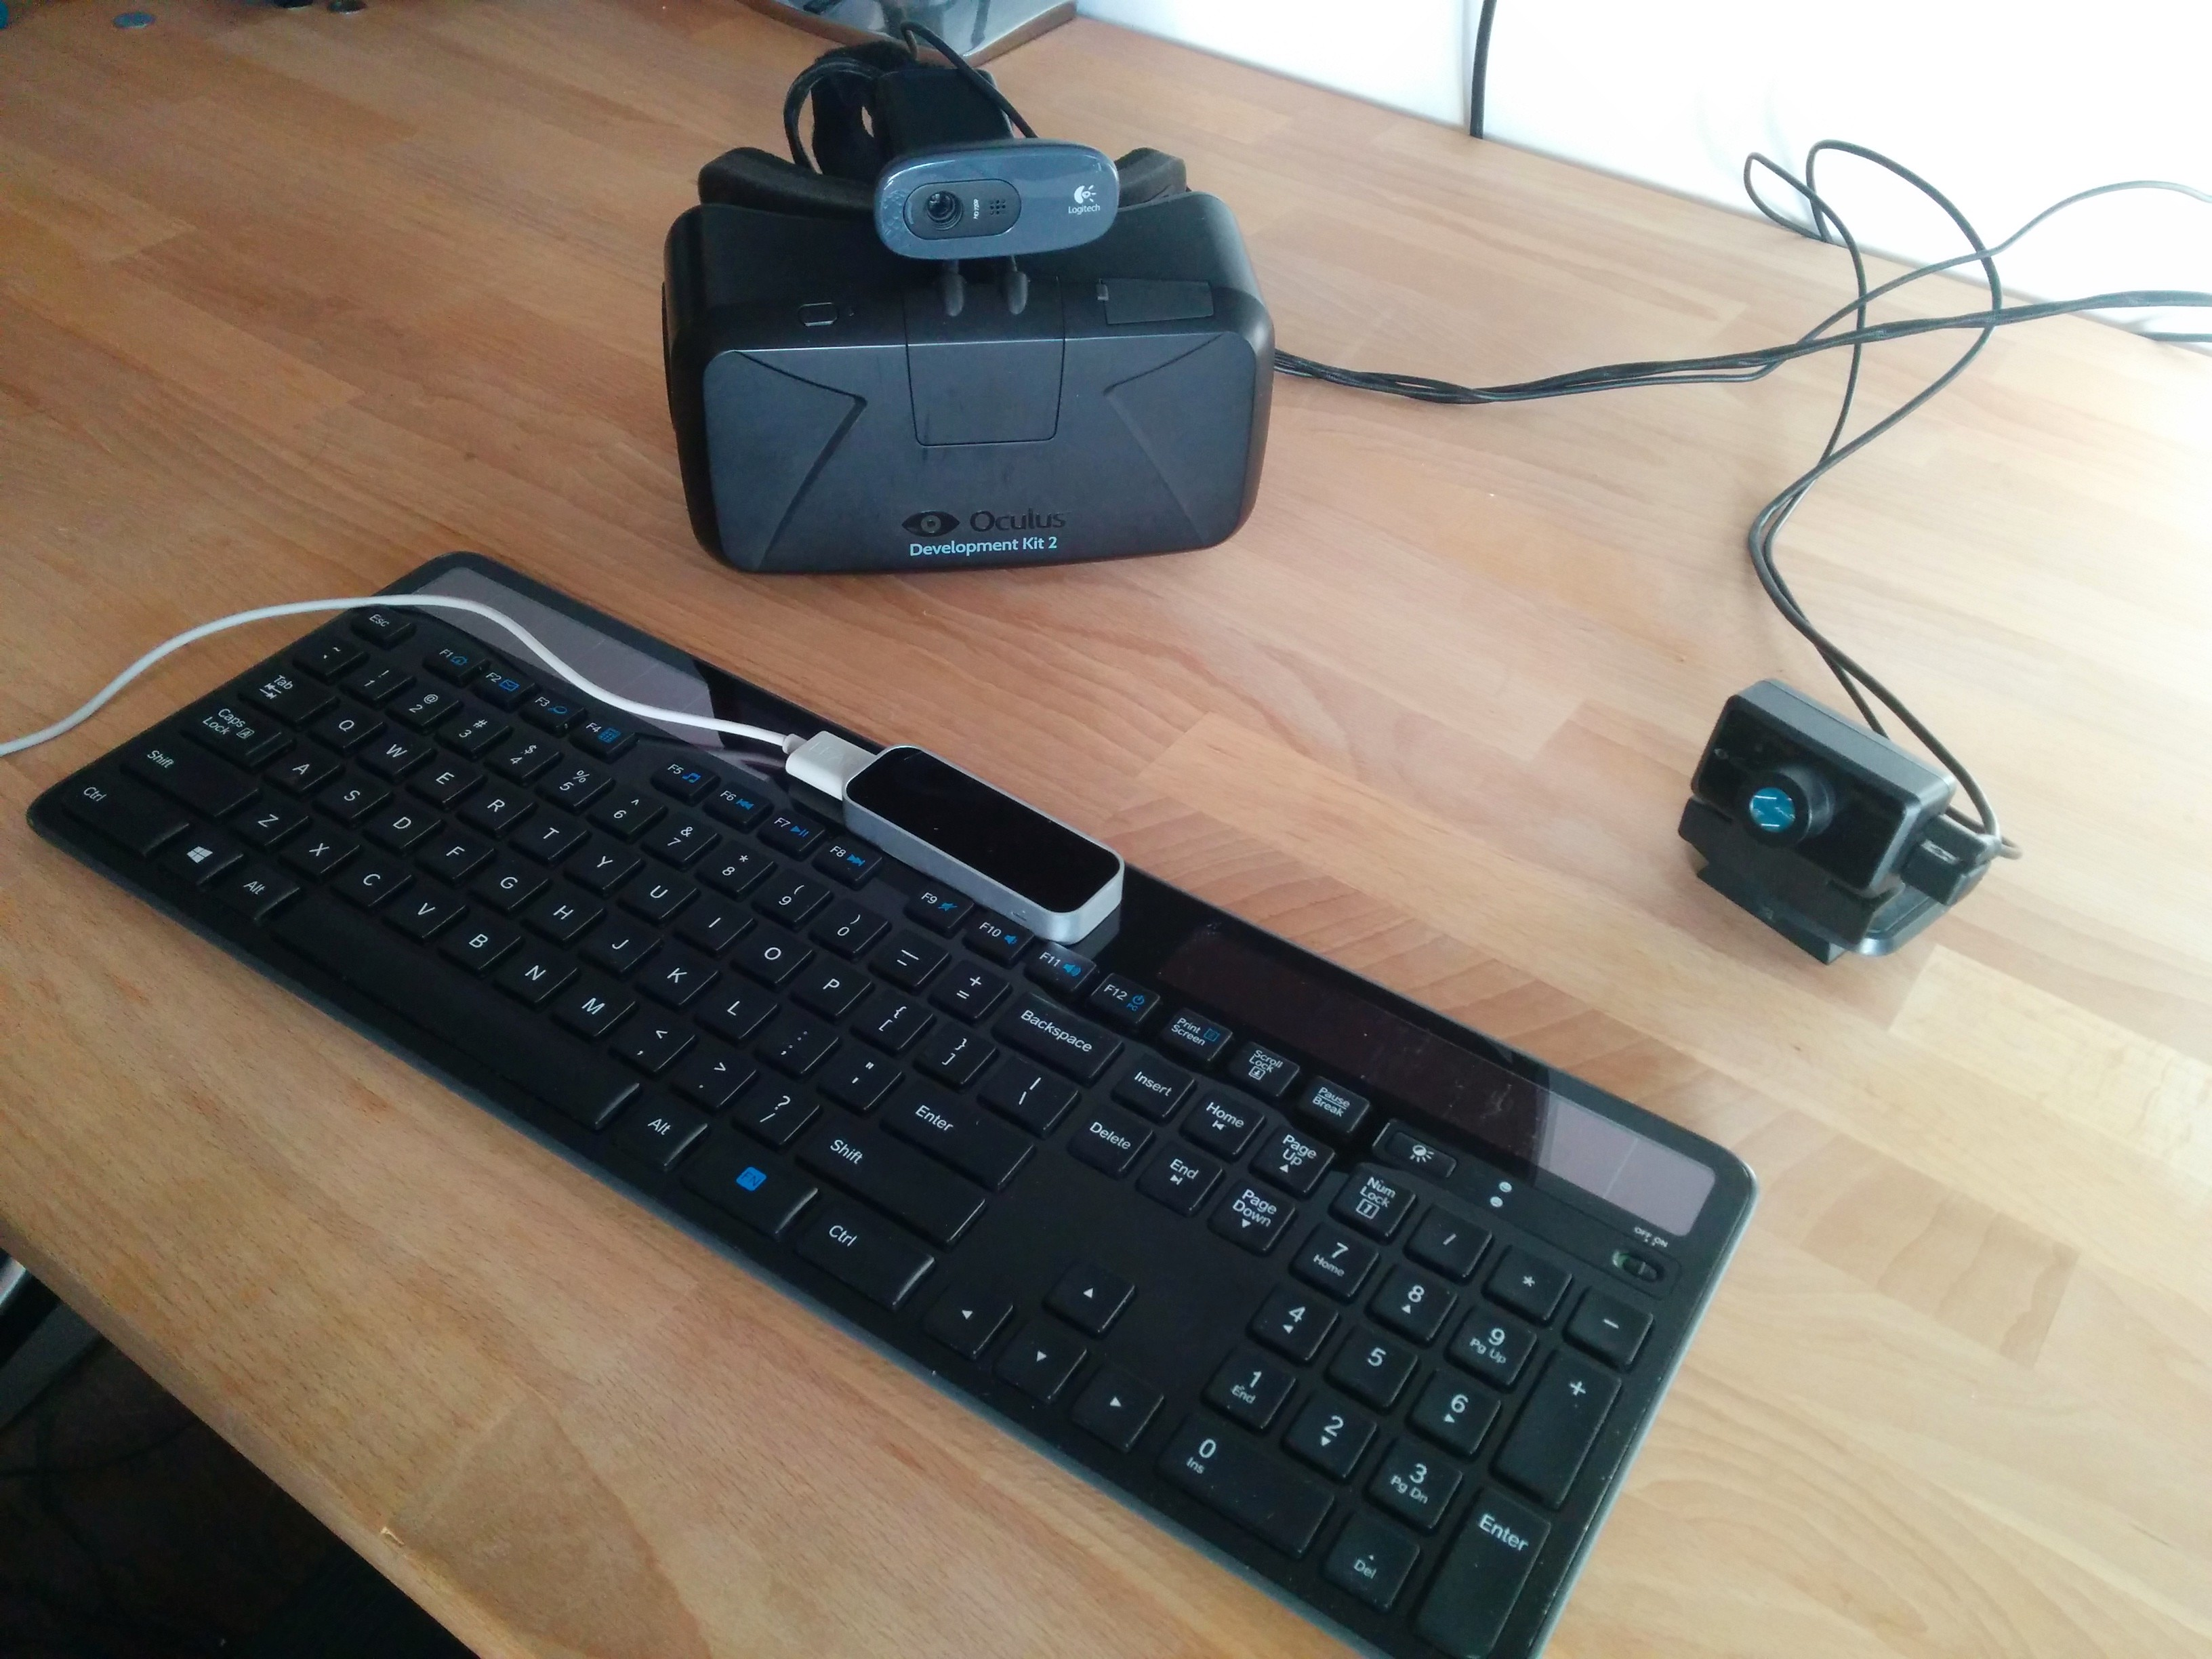
\includegraphics[width=.45\linewidth]{figures/setup/equipment}\label{fig:rift}
 	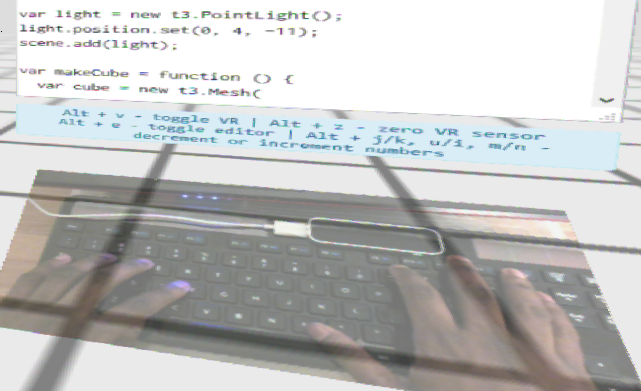
\includegraphics[width=.45\linewidth]{figures/setup/webcam_passthrough}\label{fig:leap}
\end{tabular}
\caption{Leap Motion with webcam attached to Rift (left), keyboard inside VR (right)}
%	\caption{Leap Motion with webcam attached to Rift \label{fig:rift}}
%\end{subfigure}%
%\begin{subfigure}{.5\columnwidth}
%  \centering
%  \caption{Leap Motion and keyboard inside VR \label{fig:leap}}
%\end{subfigure}
\end{figure}

% Data Mountain: http://www.microsoft.com/usability/UEPostings/p153-robertson.pdf
\emph{Affordances}, are devices that often leverage innate cognitive mechanisms when performing actions in an environment, and can result in increased task performance. 
Researchers have attempted to improve interfaces and programming environments that incorporate the human capacity for attention, cognition, and memory.
For example, in one study, participants organized their web bookmarks by positioning screenshots of the pages on various piles in a 3-dimensional space~\cite{Robertson:1998}. 
%After 6 months, participants could still recall the bookmarks based on position alone.  

Similarly, researchers have incorporated affordances for spatial memory in programming environments.  Code Canvas~\cite{DeLine:CodeCanvas} positions code files on a large scrollable plane which enables preservation of stable spatial positions of code location.  Code Bubbles~\cite{Bragdon:CodeBubbles}, allows a developer to quickly position related fragments of code on an infinitely scrollable screen, which improved navigation and comprehension of fragments.  Patchworks~\cite{Henley:2014}, removed management of fragments and introduced a more stable position, to improve disorientation that was still present with users of Code Bubbles.

\begin{figure}[ht]
\centering
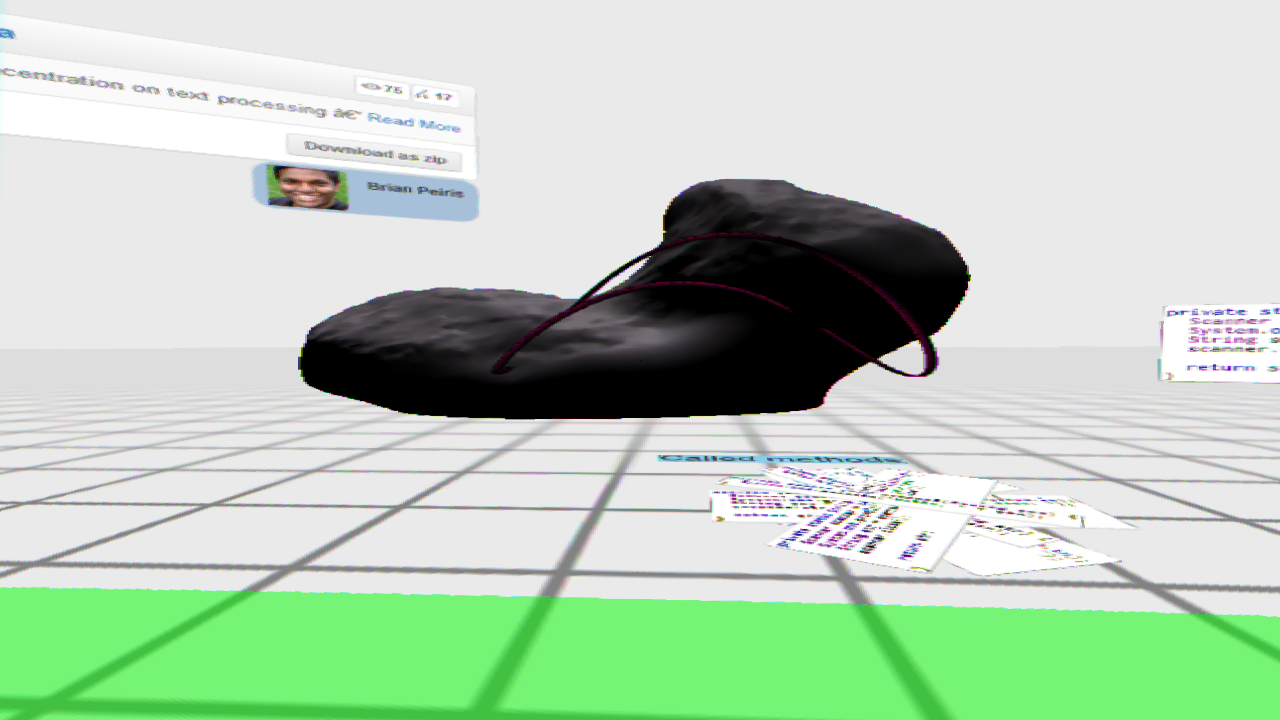
\includegraphics[width=\linewidth]{figures/unwarped_comet2}
\caption{The active fragment is in the middle of the user's view. The user is currently looking at the implementations of the methods (shown to the right) called by the active fragment. The user is able to easily read 3 of these fragments at once.  \label{immersion}}
\end{figure}

%Live feedback (update with hands).  Simulation sickness.
In this paper, we describe how head-mounted virtual reality displays coupled with gesture input devices provide several previously unexplored affordances not yet fully utilized in a programming environments. 
%Understanding the challenges and benefits offered by programming environments supported by VR is a space worth exploring.
%We then illustrate a scenario with a future programming environment that fully integrates VR.  
We then describe several systems we have prototyped and how the systems can be used in several applications related to software engineering.  Finally, We provide a brief discussion of some open research questions and discuss some of the challenges of using VR in software engineering with existing technologies.


%which enable the user to feel immersed in a virtual environment., and live feedback in the environment, 
%Our motivation and argument is simple: 
%Introducing affordances that leverage human capabilities can lead to improvements in programming environments.
%Interaction and manipulation of virtual space is a compelling but relatively unexplored alternative to windowed programming environments, with a set of new capacities to support affordances not currently available in existing programming environments.   




\section{Affordances in Virtual Reality}
% this is what VR can give that has not been captured by other domains
% go into a bit of detail for each item
% give concrete example of VR: we used the Rift and Leap Motion
% the affordances allow an immersive environment: big whoop. Why should I care about an immersive environment?
We describe a set of affordances that VR provides and describe the potential benefits of integrating them into programming environments.

\subsubsection{Spatial Cognition and Memory}

Head-mounted virtual reality displays allow the user to update their view by moving their bodies or rotating their neck, even a full 360 degrees.
Additionally, these displays render a slightly different image for each eye (stereoscopic rendering) which enables the human eye to more easily sense depth of images on the display.
%VR devices also completely immerse the user in the environment, so that the user's head has six degrees of freedom. 
Virtual reality can directly mimic the affordances offered by physical navigation. Based on electrocorticography (eCoG) recordings on the surface of the brain, the firing patterns of place cells could observed as a person navigated a virtual town and again when they later recalled the paths through the town~\cite{Ekstrom:2003}.


%VR devices render a slightly different image for each eye (stereoscopic rendering) which allows humans to sense depth in the images just like in the physical world. 
%VR devices also completely immerse the user in the environment, so that the user's head has six degrees of freedom. 
%This realistic imitation of the human body enables easier and more natural navigation as well as the ability to display more information at once in a meaningful way. 
%We get the naturalness of the physical world and the malleability of the virtual world.

%Virtual environments can use the immersive property to display more information than on a computer monitor. 
%We are still limited by the field of view of the human eye, so putting more information on the display is not novel, but what is novel is being able to distribute that information around the user in a meaningful way. 
%This immersion is possible because the Rift uses stereoscopic rendering (creates a slightly different image for each eye) to enable depth sensing.

%afforadance =>
%Data mountain. More pathways => more activation. LTP persistence. notes: predict longer term retention.

\subsubsection{Manipulation and Motion}

The affordances provided by manipulation of a physical object can result in improved perception and retention. 
For example, consider how the affordances offered by turning pages of a book result in increased comprehension and recall of the text when compared to reading on computer displays~\cite{Noyes:2008}.
Additionally, the ability to serendipitously browse and relocate material is improved.
% on paper due to the ability to turn pages.
%especially when the content is complexity.
%Objects: E-books vs textbooks.
%manipulation with leap motion.
% http://embodiedknowledge.blogspot.com/2011/12/classic-experiment-by-held-and-hein.html
Motion in a physical space, through exertions such as walking, have important cognitive consequences~\cite{Oppezzo:2014}.
%Simply going for a walk increases creativity, even prior to starting the creative task~\cite{Oppezzo:2014}.
Other affordances can be aided by motion. For example, perception of depth is enhanced by self-actuated movement in a space~\cite{Held:1963}.
%Memory...

Researchers have explored integrating natural interactions with existing programming environments~\cite{Delimarschi:2014}.
Through input devices such as the Leap Motion, it is possible to also manipulate and interact with virtual objects.
Physical movement is possible in virtual spaces.  Body harnesses\footnote{\url{http://cyberith.com/product/}}, allow free movement in a virtual space, including walking, running, and vertical movements such as jumping and crouching.%  Such devices are as affordable and require less space than standing desks.

%Self-actuated motion enhances the 

%Computer- vs. paper-based tasks: are they equivalent?
%Noyes JM, Garland KJ.
%Ergonomics. 2008 Sep;51(9):1352-75. doi: 10.1080/00140130802170387. Review.

\subsubsection{Liveness}

Liveness is a powerful affordance that can be defined by the speed and level of responsiveness to actions offered by an environment~\cite{Tanimoto:Liveness}.
The potency of giving programmers a direct and immediate connection to their creations has been well illustrated in Bret Victor's seminal lecture, ``Inventing on Principle''~\cite{Victor:InventingOnPrincipleVideo}.%\cite{Victor:InventingOnPrincipleTranscript}.

When liveness is violated, the results can be nauseating.
Simulator sickness is distinct from motion sickness, in that it arises due to a mismatch between a person's interaction and the expected response of the environment.
For example, a person in virtual reality can become nauseous when they attempt to interact with the system but the system does not respond quickly enough.
This is most apparent with head rotation, where users rotate their physical heads expecting to see an updated view but still see the initial view.

\section{Motivating Example}
% Danger of using "you", as researchers aren't programmers and sadly can't identify with this!
Consider the following scenario: A space mission has just landed a probe on the surface of a comet.
After 10 years in flight, the probe lands against all odds but in a position that is unable to receive sunlight and without deploying its anchoring harpoons.
Automated telemetry programs cannot find a feasible path. As a programmer, you are tasked with updating the lander's software to reposition itself safely on solid ground and you have 24 hours before its batteries die and the probe deflects off the comet surface. Thankfully the companion orbiter has gathered detailed information about the surface around the landing site and telemetry data shows exactly where and how the lander is positioned.

You update your simulation with the data and step into VR to survey the situation. 
After assessing the lander's options, you iterate on a number of solutions, first by using your hands to manipulate a possible path and scale thrust settings, 
and then the keyboard to refine the code. With each solution you observe the lander's behavior inside the simulation.
You walk around the lander to inspect it's position after each maneuver, leaning in to ensure that its feet are planted firmly in the regolith, zooming out to an orbital view to verify that its new position maintains a line-of-sight to the orbiter on this lob-sided comet. 

%% talk about this in remote collaboration
%A peer programmer joins and watches a replay of your live coding session.  She notes an issue with potential collision and suggests that you can correct the path by gently crashing the the companion orbiter into probe.  You add this to the simulation, it seems to work.  But you're not done yet, the peer programmer has noticed a part of the code light up in the distance.
%It is a warning that the collision detection code will not let you execute this action outside of the simulator.  You get around this by shutting off the engine right before impact.

Finally, after having run the simulation dozens of times in VR, you upload the program with time to spare. 
The lander repositions itself as expected and the historic mission can continue successfully.
  

%\section{Systems}

%We have built two virtual reality prototypes for software engineering to concretely demonstrate the affordances of VR. 
%\textsc{RiftSketch} primarily illustrates \emph{liveness} and \textsc{Immersion} chiefly demonstrates \emph{spatial cognition and memory}.
%Both systems use \emph{manipulation and motion} to aid their primary goals.
%Both of these systems use a head-mounted display (Oculus Rift - Development Kit 2) to visually immerse the user in the environment and a Leap Motion Controller for gesture recognition.
%To assist in interaction with the keyboard, we allow reality to shine through by using a web camera mounted on the Rift and project that image in the system (See Figure~\ref{fig:rift}).


%\subsection{RiftSketch}

%\textsc{RiftSketch} is a live coding environment built for VR.~\cite{Peiris:RiftSketchVideo}
%It allows a user to describe a 3D scene using geometries, materials, textures, lights, meshes and other primitives provided by the Three.js library, which is a convenient wrapper for the WebGL APIs available in modern browsers. 

%\textsc{RiftSketch} presents a user with a simple text editor, floating in front of them in an otherwise empty VR world. 
%As the user types code into the editor, the world around them updates instantly to display the 3D scene dictated by their code. 
%\textsc{RiftSketch} also allows the user to animate their scene via a callback function which is executed on every frame. 
%The user can manipulate the state of the 3D scene in this looped block of code in order to add behaviour to the objects in their scene.


%\subsection{Immersion}
%
%\textsc{Immersion} is a code review prototype that displays code fragments in multiple ways to enhance spatial reasoning.
%Software packages are represented as traversable floor sections and are color coded by the amount of code modified for this review.
%The reviewer's view is centered around the active code fragment with fragment piles on the floor that the reviewer may want to see.
%Piles have previously been shown to effectively engage spatial reasoning.
%The reviewer is able to expand one pile at a time into a ring of fragments to see the details of the fragments, based on Schneiderman's taxonomy including overview and detail visualizations~\cite{Shneiderman:InfoVisTaxonomy}.
% I looked at Code Canvas, but they didn't cite anything for semantic zoom
%\textsc{Immersion} uses semantic zoom to make method names readable even when at the back of the ring and the fragments retain a scaled height enabling the reviewer to approximate its length. 

%In the following section, we more fully describe how both the \textsc{RiftSketch} and \textsc{Immersion} systems demonstrate the benefits for software engineering by using the affordances of a VR environment.

\section{Applications}

We have built two virtual reality prototypes for software engineering to concretely demonstrate the affordances of VR.
In this section we describe how these systems can provide affordances and interactions from the comet example above in live coding and code review.

Both of these systems use a head-mounted display (Oculus Rift - Development Kit 2) and a Leap Motion Controller for gesture recognition.


\subsection{Live Coding}

\textsc{RiftSketch}\footnote{http://www.youtube.com/watch?v=SKPYx4CEIlM} is a live coding environment built for VR which allows users to describe a 3D scene using the Three.js library\footnote{http://threejs.org/}.
%It allows a user to describe a 3D scene using geometries, materials, textures, lights, meshes and other primitives provided by the Three.js library, which is a convenient wrapper for the WebGL APIs available in modern browsers. 

\textsc{RiftSketch} presents a user with a simple text editor, floating in front of them in an otherwise empty VR world. 
As the user types code into the editor, the world around them updates instantly to display the 3D scene dictated by their code. 
\textsc{RiftSketch} also allows the user to animate their scene via a callback function which is executed on every frame. 
The user can manipulate the state of the 3D scene in this looped block of code in order to add behaviour to the objects in their scene.

To assist in interaction with the keyboard, we allow reality to shine through by using a web camera mounted on the Rift and project that image in the system (See Figure~\ref{fig:rift}).

\begin{figure}[ht!]
\centering
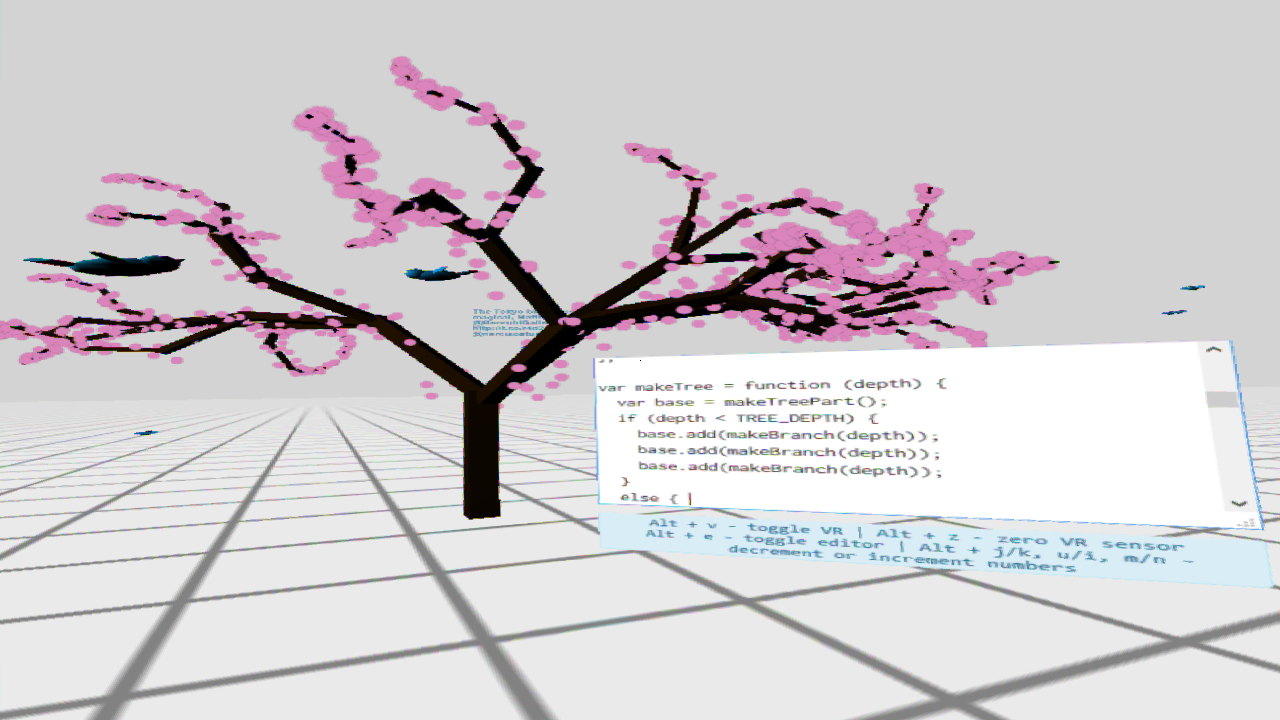
\includegraphics[width=80mm]{figures/riftsketch/unwarped_tree}
\caption{\textsc{RiftSketch} screenshot. The tree is generated by a recursive algorithm that the user has typed into the floating editor. The flying, animated birds represent tweets pulled in from the Twitter API, also generated by code that the user has entered. \label{RiftSketch}}
\end{figure}

\subsubsection{Liveness}

\textsc{RiftSketch} demonstrates liveness by providing a tight feedback loop between code written and its effect in a virtual environment, and to quickly experiment with various solutions, algorithms and calculations. 
\textsc{RiftSketch} is also very promising as a learning tool since users can see their mistakes immediately and correct themselves without an intermediate compile step that might otherwise act as a hindrance.  
These benefits are especially evident in \textsc{RiftSketch} when the code describes a VR scene. 
Watching the entire virtual world change around you as you type can be an extremely powerful and engaging experience.

\subsubsection{Hand Manipulation of Code}

Furthermore, \textsc{RiftSketch} provides the user with shortcuts and input methods to quickly edit numbers in the code that they write. 
Keyboard shortcuts allow the user to increment or decrement numbers in the code by factors of 0.1, 10 or 100. 
Integration with the Leap Motion Controller provides users with the ability to manipulate numbers using natural input: the user places the editor's cursor over a number and then can move their hand up and down above the Leap Motion controller in order to increase or decrease the number. 
Numbers in the code could represent anything, from the X, Y or Z components of a position or rotation vector, the red, green or blue components of an object's material or a component in the calculation of an object's animated speed.


\subsection{Code Review}

\textsc{Immersion} represents methods as code fragments similarly to Code Bubbles~\cite{Bragdon:CodeBubbles} and displays groups of fragments as piles on the floor like BumpTop~\cite{Agarawala:BumpTop}.
Piles can be expanded into a more detailed ring: an overview and detail visualization~\cite{Shneiderman:InfoVisTaxonomy}.


\subsubsection{Spatial Reasoning}

The reviewer initially sees the active fragment in the center of the screen with other relevant fragments distributed around the floor in piles. 
Reviewers use spatial cognition to judge the relevance of piles by how far away the pile is as well as the size of the pile.
The reviewer is able to scan the labels of the piles and number of fragments in each pile to quickly verify if each pile is indeed relevant.

\textsc{Immersion} divides the floor into sections based on packages of the system and color codes the sections to indicate how much that package has been modified by the code under review.
By walking between packages, we expect reviewers to have better mental models due to the increased usage of spatial reasoning.
Similarly, we expect that reviewers would be able to more easily recall review details after the review since the spatial elements of their brains were more engaged.

%Info displayed up/down, left/right, forward/backward.
%Uses all three dimensions. 
%Code Canvas and Code Bubbles could only allow two dimensions.

\subsubsection{Gesture Interaction}

Reviewers can make a grabbing motion to select a pile and then can pull their hand up to transform the pile into a ring of fragments for more detailed inspection.
The reviewer is now able to read the foremost fragment in the circle and can make horizontal finger swipes to rotate the circle and read other fragments. 
The reviewer can pinch the foremost ring fragment on the top and bottom and move it to the middle of the screen to become the active fragment.
The piles then change to include code relevant to the new fragment, but the reviewer can move their hand as if clearing off a desk to return to the previous active fragment if they want to go back.

% Imagining room inside HiFi with multiple avatars
% each developer could have an avatar
% able to get facial expressions
% able to get body language (although somewhat expensive right now, these prices will come down)

% able to sense body language in real time
% able to hear in real time
% environment is dynamic

% pair programming
\section{Discussion}

\subsection{Future Directions}

\subsubsection{Simulation}

Virtual reality is well-suited to applications with physical analogs that can be simulated in 3D such as the earlier comet example. 
Although simulation software is not uncommon, 3D worlds and models are often difficult to navigate and interact with when displayed on 2D devices. 
Users have to actively think about moving a camera viewpoint in 3D space in order to view a certain part of a simulation. 
%Interacting with a simulation might require positioning a virtual cursor which can be challenging when you only have a 2D view of the scene. 
% TODO - relate to comet

%VR, on the other hand, allows users to view, explore and manipulate simulated worlds directly. One can imagine a user physically turning their head to look around a simulated car plant or using their hands, via a Leap Motion controller, to interact with a simulated robot. 
%These direct interactions provide a subtle but important advantage over 2D-projected simulations. 
%This sense of immersion gives the users unimpeded access to the simulation which allows for quicker turn-around when testing or debugging the simulated software, especially if combined with an in-situ live coding solution like \textsc{RiftSketch}.


\subsubsection{Remote Collaboration}

Both \textsc{RiftSketch} and \textsc{Immersion} could help facilitate remote collaboration.
Multiple programmers located around the world could join each other in a VR live coding space to figure out how to land the comet from the motivating example.
They would be able to provide extra insight and could arrive at the solution faster.

A different set of programmers, also located around the world, could then join each other in a VR code review environment to review the proposed solution.
They are able to see what each person is thinking based on their annotations of the piles of information in their section of the system.


%Co-located development teams are able to communicate in person. 
%Distributed teams can try, but the technology is too slow and it doesn't feel right. 
%High Fidelity \footnote{https://highfidelity.io/} is implementing infrastructure for virtual worlds that is fast enough for developers to be able to sense body language and hear audio in real time.  
%Distributed development teams will have the foundational issues of remote communication solved which enables a shared VR environment to become truly powerful.

%A benefit of co-location is pair programming, where two developers program at the same computer and can catch each others errors. 
%VR and body sensing with a device like PrioVR would enable remote developers to be at a shared virtual desk right next to each other. 
%They would be able to see the same files, talk in real time, and even point to which line of the code they are talking about. 

% pair 'live coding'/code review
%Sharing a live coding environment enables all participants to have a tight feedback loop. 
%This could be especially useful when the primary developer of a section needs to explain their modifications to the rest of the team. 
%Everyone could meet in the shared VR live coding environment and watch while the developer walks through modification of their code. 
%The team would be able to see how the system changed rather than looking through large amounts of code.

  % pair designing
%Co-located teams can design together around a whiteboard in a conference room as they talk through the problems of the system. 
%A shared VR environment could have a similar room with sketching space that everyone can see. 
%Developers could drag-and-drop files or code snippets to display on the walls around them. 
%They could then discuss and annotate the code. 
%Additionally, visualizations such as structure diagrams or architecture of related systems could be overlaid on a wall for reference.

% exploring data visualization together
%Remote workers could experience immersive visualizations together. 
%A control flow graph could be represented by a maze of rooms through which the team could walk. 
%The team members could trace different paths and yet still be shown an overlay of where each of the other members are and how these positions relate to each other. 
%Currently remote workers can each trace separate paths of the code but have a hard time communicating what those paths are and how they relate to each other.

%Remote workers often miss out on many benefits that in-person communication can bring. 
%Shared VR spaces tailored to developers' activities can fill some of the gaps caused by distance and help the team to function better together. 


% git diff + complexity vs active fragment
%\subsubsection{Big Picture}
%\textsc{Immersion} also displays overview diagrams of this changeset to allow the reviewer to see where this active fragment fits into the changeset as a whole. 
%Similarly an overview of the cyclomatic complexity also helps the reviewer to see which areas of the code would be most relevant to see. 
%These diagrams illustrate how VR is able to show multiple overview and detail diagrams without overwhelming the user.

%Immersive VR environments have a lot more space for information display than current computer workstations.
%We used \textsc{Immersion} to illustrate that VR software engineering tools can use this increased space and the affordances of VR to more easily analyze and navigate the displayed information.
% What does VR provide that makes this different from using a Leap with 5 monitors?


%\subsection{Simulation}

%\section{Discussion}
% VR vs AR in the future, which is better?
  % code snippets while wearing Google Glass could appear on peripherals
%We have presented two systems with applications in software engineering.

%Although the current implementation of \textsc{RiftSketch} is little more than a creative toy, the authors' experience of using it for dozens of hours shows the potential of future applications. 

%In practical applications, one could extend the concept of live coding and tight feedback loops in order to create customized programming environments. 
%VR programming environments could allow the user to take advantage of the malleability and expanse of virtual worlds. 
%For example, a user could live code a widget that indicates some statistic of the code they are currently editing, such as the cyclomatic complexity, test coverage or test result. 
%The widget would update itself as the user typed, not unlike existing code feedback tools such as NCrunch \footnote{NCrunch automated concurrent testing tool: http://www.ncrunch.net/}, and they could position the widget in their virtual periphery.

%\todo[Anthony]{Opportunities for other gestures: Refactoring}

\section{Open Questions}

\subsection{Degrees of Immersion}

Augmented reality devices such as Google Glass, aim to help the user complete tasks in the physical world by adding information overlays. 
Augmented reality seeks to help the user in the physical world while virtual reality seeks to completely replace physical reality. 
\emph{Is it more useful to immerse the user in a completely virtual environment, or to enhance their physical world?}

% Where is the limit for too much info displayed at once?
%\subsubsection{Information Overload}
% Somewhat discussed by Healey 2006: http://www.csc.ncsu.edu/faculty/healey/download/apgv_volume.06.pdf
%A large advantage of VR is being able to display more information at once to the user.  
%At what point does the extra information cause overload and begin to hinder productivity?  
%Is this balance between amount of information and processing speed the same for each person (other aspects of VR can differ per person)?

% Does using a VR code review tool actually increase comprehension? Does it allow users to find bugs and provide alternative solutions?

% What gestures are most natural in VR?
\subsection{Input Forms}
Gaming console controllers work well for navigation and limited action support but are surpassed by keyboards at text entry.
However, such devices require users to interact with both the physical and virtual worlds at the same time.
Gesture recognition removes interaction with the physical world but can cause physical strain.
Voice recognition could reduce strain but may feel awkward in a shared work space.
\emph{What is the best way for the user to provide input to a VR system?}

\section{Challenges}

\subsection{Separation from the Physical}
Putting on a VR headset means blocking out the rest of the physical world, including coworkers.
Peers may lack the opportunity to ask questions and physical communication is stifled.
Additionally, the VR headset wearer may have trouble interacting with the physical world while in VR.
A webcam mounted to the headset enables some interaction with the physical world, as seen in Figure~\ref{fig:rift}, but has a limited field of view.

\subsection{3D Mapping}
Some problems don't have an inherent 3D representation which makes display in VR a challenge.
As seen in \textsc{Immersion}, 2D code can be displayed in VR but the code itself does not have a third dimension and thus loses the expressiveness of 3D.
This could be an area well suited to 3D metaphorical programming as suggested by Ko et al.~\cite{Ko:LearningBarriers}.

\subsection{Technology Limitations}

The 1080p resolution of the Oculus Rift Development Kit 2 allows for passable text reading, but needs improvement for multi-hour sessions. 
The Rift also requires users to measure the distance between their pupils for more accurate stereoscopic rendering, but current utilities are either time consuming or hard to use properly.
Eyeglass wearers must go through extra trial and error to see if the headset is best used with glasses on and a reduced field of view or replace their glasses with stronger lenses in the Rift and have increased blurriness.


\section{Conclusions}
%We have shown that virtual reality enables a new interaction paradigm that can improve developers' lives. 
%The immersive environment allows users to process more information at once and stereoscopic rendering enables depth-sensing. 
%Together, these affordances provide a novel platform for new software engineering tools.

We envision a future where software engineers work in immersive environments which take advantage of more affordances of the human body than current workstations.
We argue that these affordances provide a platform for new kinds of software engineering tools. 

%We imagine a future in which many software engineers find it most productive to design and build software within a VR environment. 


%%%%%%%%%%%%%%%%%%%%%
%%%% NOTES
%%%%%%%%%%%%%%%%%%%%%

%We describe our vision of what software engineering would look like with VR by illustrating various principles across four different immersive VR environments.
%First, we show how an immersive code review environment could enable software engineers to more easily analyze and navigate information which leads to increased understanding of the software. Secondly, we show how an immersive live coding environment could enable much faster development times when creating 3D scenes.
%Next we show how a social immersive environment could improve communication among remote development teams.
%Finally, we show how an immersive environment could be used to experience physical analogs of abstract software.
%We provide a brief discussion of some open research questions and discuss some of the challenges of using VR in software engineering with existing technologies.
%[Discussion]

%(stable locations), code bubbles (quick associations), patchworks (reduce view management issues in code bubbles).

%Andrew Bragdon has implemented a system called Code Bubbles that enables the user to pull out methods from a file. 
%The user is then able to move and group the methods as desired.  
%Code Bubbles also can display the call graph for the selected method and allows the user to open called methods.

%Code Canvas added semantic zoom to the Code Bubbles tool, allowing the user to gain a better understanding of how the current section of the system fits into the system as a whole~\cite{DeLine:CodeCanvas}.
% lacked a set of rich and stable environmental cues.

%Place cells, navigation, Kuhn (natural). Disorientation here.  Research has gradually introduced solutions that incrementally introduce elements that improve spatial memory support in programming environments (Desert, code canvas, code bubbles, patchworks, etc).  But where is the design ultimately heading?

%Understanding, navigating, and changing software systems is daily challenge for software developers.

%a main window for viewing content with a set of navigational links (tabs, tree views, and search results) to allow transitions between content.  
%Research advances: More advanced forms allow multiple fragments or windows software to be displayed at once.

%but limited design choices and increasing 
%scale of development efforts grate against these capacities.  
%Spatial memory.  Kuhn.

% http://www.scientificamerican.com/article/reading-paper-screens/
% http://healthland.time.com/2012/03/14/do-e-books-impair-memory/

%The choices developers have available so far is to choose between better links to software while coding in a main document (e.g. recommendation systems)
%or showing all the software (never escaping some form of view management due to the limited space to display content).


%The motivation for these approaches (spatial memory).

%Developers spend a large amount of time navigating source code.
%In a laboratory study of 10 experienced Java developers, Ko. Developers spent, on average, 35 percent of their time performing the mechanics of navigation within and between source files. Previously, I studied data~\cite{Parnin:2006b} from twelve programmers collected over several months of development activity in the professional workplace and found that developers work with 57--83 methods in a day (25\% and 75\% percentile respectively) and frequently switched between those methods as they worked. 60\% of transitions were to different classes.

%Observations of developers suggest they frequently rely on associations with \emph{environmental cues}\textemdash interface elements of the programming environment\textemdash 
%for navigating and understanding new code.  For example, Ko et al.~\cite{KoMaintenance06} observed that programmers use cues, such as open-document tabs and scrollbars, 
%for maintaining context during their programming tasks.  However, these cues are often insufficient: The act of navigation often disturbs the state of environmental cues, 
%and the paucity of interface elements, such as tabbed panes, which often only contain a file name, starves associability.
%In studies of developer navigation histories, a common finding is that developers frequently spend time flipping through open tabs because they fail to associate the tabs with desired code locations~\cite{Singer05}.

%Interactive displays of various sizes and form can greatly expand the mental workspace of developers.  
%Pulling aside a particular item of interest can be far easier and less costly than managing everything as a fragment or hoping for an 
%intelligent heuristic to provide access to the correct artifacts.

%[Applications of VR in software engineering]
% This section could be said in better words or bullet points, or VR, or *something*


\bibliographystyle{abbrv}
\bibliography{nier2015_Immersion}
\end{document}
